\documentclass{report}
\usepackage[utf8]{inputenc}
\usepackage{graphicx}
\title{User Manual}
\author{Oscar Daniel}
\date{February 2015}
 \graphicspath{ {Images/} }
\begin{document}
 
\maketitle
 
\tableofcontents
 
\chapter{This Product}
 This product is a revision and teaching aid for A Level science subjects, allowing teachers to set their students questions and allow the students access to as many questions as they like. The GUI of this program is designed in a way to allow a user of any technical ability to easily understand and make use of the program.\\
 The program works by all users having a copy of the "Teaching Aid.py" file on their work stations and a file that every station can read and write to, through the program, containing the pickle files storing user and question data.
 


 
\chapter{Installation}
 All computers that will use the program need to have Pyton 3.4 and PyQT 4 installed on every machine that will run the program.\\
 Python 3.4 can be found here : https://www.python.org/downloads/\\
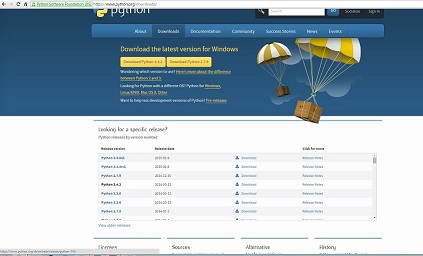
\includegraphics{PythonDownload}\\
 \clearpage
 PyQT 4 can be found here: http://www.riverbankcomputing.com/software/pyqt/download\\
 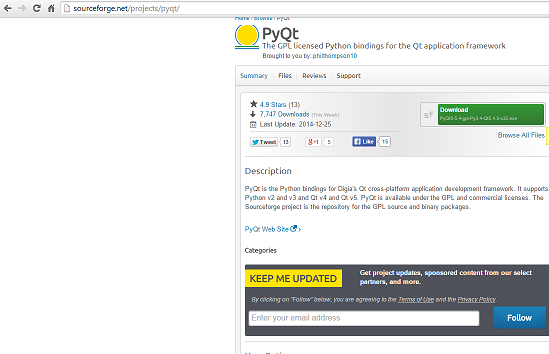
\includegraphics{PyQTDownload}\\
Follow the installation wizards to complete the installations.
Only Python version 3.4 and compatible versions of PyQT will work with this program code. Please ensure that you have installed valid distributions before continuing.\\
 
 
\chapter{First Time Setup}
\section{Moving The Program Files}
To ensure that the program will run as effectively as possible, you will need to put files in the correct places.\\
The "Admin Tools.py" file will need to be placed in a file that you wish your users to be able to read and write to, regardless of which workstation they are using. i.e. a shared drive.\\ \textbf{Important:} When you have done this, copy the file path of your "Admin Tools.py" and add it to the subroutines in the "Teaching Aid.py" file in your program folder, as shown below:\\
\textbf{Warning: }If you do not do this before copying your "Teaching Aid.py" file you will need to repeat the last step for each file on each workstation.\\
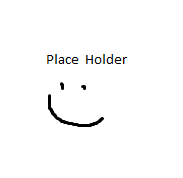
\includegraphics{placeholder}\\

The modified "Teaching Aid.py" file will now need to be placed on every workstation, in a place where any user can access it.
\section{Admin Tools}
After installing the necessary programs, you will want to run the "Admin Tools.py" file. You then need to create an admin account by filling out the form and pressing submit.\\
\inludegraphics{adminlogin}\\
\textbf{Important: }You should store these credentials somewhere secure as you will need them to access the Admin Tools again.\\
 Once you have done this you will need to run each of the "create / clear" routines for pickle files by clicking the buttons labelled such.\\
 
\textbf{Warning: }If you do this after editing these files, any changes will be deleted.\\
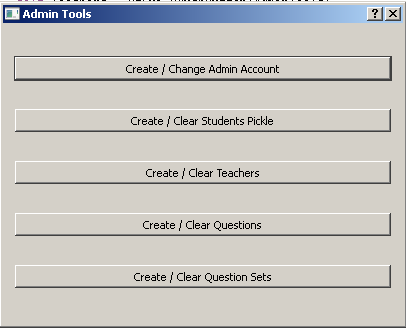
\includegraphics{AdminTools}\\
\chapter{Adding New Users}
Now that you have completed your first time setup, you will need to add all of your required user accounts. These steps can be done at any time using admin or credentials.\\
To add new users to your program, you will need to open a "Teaching Aid.py" on a workstation which meets all pre-requisites and login with the Admin or a Teacher account:\\

\bigskip

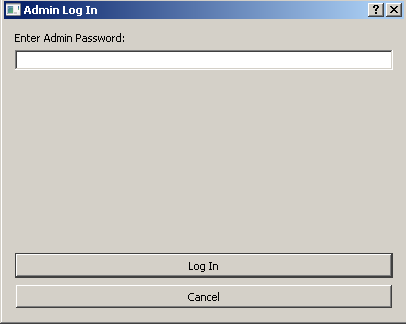
\includegraphics{adminlogin}\\
\bigskip

\bigskip
Then click the "Add New Account" button on the main window:\\
\bigskip
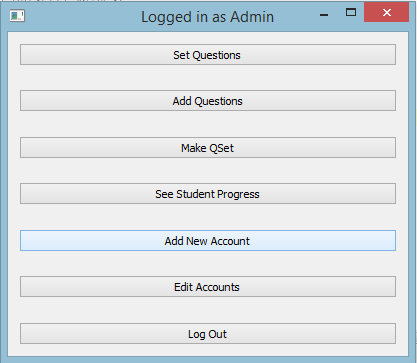
\includegraphics{adminmain}\\
\clearpage
From the create account window you are able to add new accounts to the "students.pickle" or "teachers.pickle" files.\\
However you will not be allowed to use the same username multiple times, or have a Target Grade that is not a capital letter A - U inclusive. If these are entered a dialog box will open, informing you of the error and allowing you to correct the mistake.\\
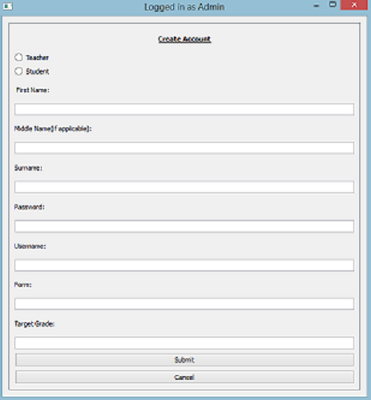
\includegraphics{addaccount}\\

\chapter{Teacher Accounts}
Teacher accounts have the ability to add questions to the question database, make question sets which they can then set pupils to do, see students' progress and create / modify accounts. \\
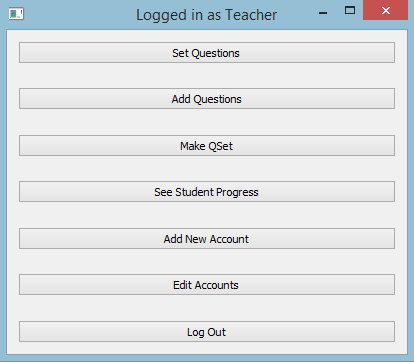
\includegraphics{teachermain}\\
\emph{The Teacher Main Window}
\section{Making Questions}
To create new questions, click the "Add Questions" button on the teacher main window and this window should open:\\
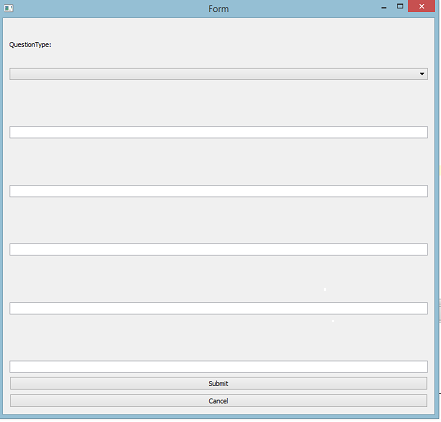
\includegraphics{MakeQ}\\
To make a new question, select a question type from the drop down box at the top of the screen, enter in values into the boxes that appear and click submit.\\
If this is done correctly a dialog box will open informing you such. If not, a dialog box will open, informing you of an error and allowing you to correct the mistake.\\
\section{Making Question Sets}
\section{Setting Pupils Questions}
\section{Reviewing Pupil Accounts}
\section{Modifying  / Creating Accounts}
\end{document}